\documentclass[11pt, oneside]{article}
\usepackage{graphicx}
\begin{document}

\title{Crimsas \\ A Text Editor with a ``Dream'' Interface}
%Crimsas stems from the color crimson, to which I randomly associate myself (my computer's name is ``Crimson-Mint") and my last name, which means Strawberry in the Scottish language. Strawberry was then translated to Spanish as Fresas, which my brother made his Xbox gamer tag. I later made my gamer tag similar with Fresas in the name. Thus, Crimsas. In case anyone was curious.
\author{Michael Fraser}
\maketitle

\tableofcontents

\section{Background}
Common text editors have many of the same features, like language-specific keyword highlighting, automatic text indentation, and easy customization. These editors often use a system of menus and forms to allow the user to modify preferences, manage the file, or access additional tools. As with most applications, the text editors also allow the user to directly manipulate the shape of a session window, the location of the session window, and the positioning of session tabs. Most of the actual text writing is done by the typing of a keyboard, with no alternative forms of text input. Text editors are very commonly used by programmers, as they offer wide ranges of file types and programs do not require the unnecessary font editing capabilities of a word processor. An ideal text editor would likely cater to programmers as much as it does to nonprogrammers.

As all text editors have many of the same features, they all maintain similar levels of efficiency, learnability, rememberability, errors, and satisfaction. The menus and forms that allow the users to easily find a desired command or tool allow for easy learnability of the editor. It also eliminates some need for high rememberability, as the forms and menus allow for commands to be quickly found again. The editors achieve similar levels of efficiency with the forms and menus, requiring several steps to reach each command. They also allow more experienced users to utilize increased efficiency with keyboard shortcuts. Satisfaction levels for the editors rely on the features of the editors and the ability for users to edit their preferences, and vary from editor to editor. As these text editors rely on keyboard shortcuts or mouse clicks to evoke commands or select tools, there is a chance for error like a misclick or pressing the wrong keys. 

Many aspects and features of today's common text editors would be included in a the design of an ideal text editor, but current text editors lack several features that could bring text editing to a new level. As new technologies are developed, new methods of interaction are developed that could alter the way text editors allow for text to be input to a document. Text editors could even take some features of common word processors to make their use as programming tools more effective and satisfying. 

\section{Designing a New Interface}
\subsection{Aspects from Common Text Editors}
While common text editors may not be the most ideal text editors, many features they have will be utilized in making a new interface. Several aspects of common text editors will be present in Crimsas, as they are steps towards an ideal interface. These features include the menus in the toolbars, keyboard shortcuts, direct manipulation of window size and position, and easy customization. 

\paragraph{Menus}
A menu system similar to the system shown in Figure \ref{Gedit_menu} will be incorporated into Crimsas. These menus allow new users to easily search through all the available commands and tools, and limit the necessary memorization of a user. Keeping the forms and menus also allows new users to be more comfortable with Crimsas, as there will be a feature they recognize from other editors they may have used. 

\begin{figure}
    \centering
    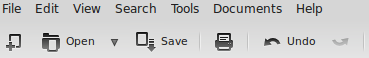
\includegraphics[width=.8\textwidth]{photos/typical_menu.png}
    \caption{The Menu Toolbar for Gedit}
    \label{Gedit_menu}
\end{figure}

\paragraph{Keyboard Shortcuts}
Keyboard shortcuts offer increased efficiency with utilizing tools and evoking commands, as they eliminate the need to search through the menus and forms to find the command or tool. Being able to quickly issue a command adds to user satisfaction as well, as the user can accomplish tasks without having to move their hands away from the keyboard. The keyboard shortcuts also provide consistency between different applications, as the many keyboard shortcuts are standard with many applications.

\paragraph{Window Sizing and Positioning on Click}
As with most applications, mouse clicks and mouse drags allow the user to modify the size of an application window, the position of the window on screen, and the organization on tabs, if applicable. This direct manipulation aspect gives the users a sense of direct control over the application. Any increased sense of control contributes to the satisfaction of the user, and so this feature continues to be in each new application. Keeping this feature also maintains consistency with different applications, so the user will expect the feature to be included.

Common symbols connected with these features include slashed lines on the corner of a window, to illustrate the window being dragged into a large window size, along with the cursor changing to a symbol indicating the edge of the window is modifiable. The symbols indicate to the user that the edge is draggable without the application explictly saying so. An example of the symbol can be found in Figure \ref{corner_symbol}.

\begin{figure}[h!]
    \centering
    
\includegraphics[width=.3\textwidth]{photos/corner_symbol.png}
    \caption{Example Corner Symbol Indicating Resizing}
    \label{corner_symbol}
\end{figure}

\paragraph{Easily Variable Preferences}
A feature that is becoming more common with applications is the easy customization of the application. When it comes to text editors, preferences such as text color, background color, indentation rules and more can be modified through a preferences option in the menu toolbar. This allows users to find a color scheme and settings they are comfortable with, and the users are able to make the application more personalized and unique to themselves. 

\subsection{New Features}
\paragraph{Voice Recognition and Input}
Text editors limit the forms of input that can be used to modify the content of a document. They also limit the way commands and tools are selected or evoked. The ideal text editor would allow multiple forms of input and command selection, and natural language is an interface style that common text editors have not explored deeply. This feature would allow the user to produce documents without having to utilize their hands much at all. As many devices are already equipped with built-in microphones and secondary devices are readily available for other devices, natural language input is easily accessible. 

This feature would never fully be deactivated unless the user has specifically disabled the feature, and would consistently be in a sort of ``wait state'' that the feature utilizes. During that ``wait state,'' any voice input will be processed and words will be matched to libraries that can then be added to the document. This feature would eliminate some need of the keyboard, and provide a new form of content input that would make the application more flexible than other text editors. In a manner similar to the Xbox One Kinect system, where keywords alert the system to behave in a specific manner, this system would utilze a keyword that allows the user to say the name of a command or tool. The system would then evoke or select that command or tool for the user, with the user needing to search through menus and forms or utilize a keyboard shortcut. To ensure the keyword does not overlap with a potentially desired word input, the keyword needs to be unique to the application. For example, the Xbox One Kinect System waits for the word ``Xbox'' to be said, which is unique to the Xbox system \cite{Xbox}. Saying the name of the application, ``Crimsas,'' will cause the system to wait for a command or option. This includes allowing for the input of special characters or telling the application to modify the file. For example ``Crimsas character comma'' will input a `,' character into the document. Alternatively, saying ``Crimsas save'' will save the file.

\paragraph{Language Libraries and Autocorrect}
Another new feature that this text editor will utilize is commonly found amongst word processors: autocorrection. Autocorrect features note when the user has made a typing error and fix the error automatically. This is done by comparing the mispelled word to the words of a word library. The word in the library with the closest resemblence to the mispelled word is then switched in to replace the mispelled word. In the event that the resemblence of any word in the library and the mispelled word does not reach a certain threshold comparison level, the autocorrect function would instead highlight the word and offer suggestions to replace the mispelled word when the user investigates the highlight. 

Autocorrecting is mostly used for spoken language corrections, but libraries corresponding to programming languages can be utilized to allow this feature to apply to a wide variety of programming languages. This will allow users to build programs with greater accuracy the first time they write the program, eliminating some errors that would need to be cleaned through debugging. For variable names, which will not match the words of a language library, placing a special character like a ``/textforwardslash'' before the variable name will shield the variable name from the autocorrect function. The special character will depend on the language being used, so as not to interfere with the program itself. The user will also have an option in the menu to select a special character to fulfill this purpose.

\paragraph{Autocomplete}
An autocomplete feature will add a new level of ease when it comes to adding content. As with bash commands in a terminal, the user will have the option to ask the program to complete the word that is currently being input (when the input is from the keyboard). The autocompletions will depend on the language being written, which will be autodetected by the application or manually set by the user. To utilize the autocomplete feature, and to stay consistent with other applications with the same feature, the ``Tab'' button will be utilized. Tab already has a special use in indentation though, so the autocomplete shortcut will be ``Shift + Tab." Adding an autocomplete function to the text editor will eliminate some need to remember all the vocabulary of a programming language, making it easier for a user to write code efficiently. The increased efficiency, along with lowering the need to consult documentation, will improve the satisfaction users have with the application. 

\subsection{Layout Features}
\paragraph{The Toolbar}
A search bar will be provided to allow users to search for a command or tool specific to the application, while allowing for the option to search a specific programming language's library for a keyword. This provides another way for the user to find a command, without them having to search through the menus and forms or remember the shortcut. 

Any buttons in the toolbar will be given wide borders of operation, allowing the user to click anywhere near the option's text or icon to access the tool or command. This aspect apeases Fitz's law of user interaction, as the larger the button is the easier the button is to press, making the task of selecting a tool more efficient. The button's will utilize icons that greatly correspond to the task or action they represent. The affordances of those icons will suggest to the user what it is that the button represents without the application needing to explicitly state the button's purpose. In the event the button's icon does not provide a clear picture of the tool it represents for the user, hovering a mouse over the icon will create a pop-up message with the command or tool's name. This pop-up message is a small assisting feature to help new user's around the application.

A tab system will be included as one of the toolbars, allowing users to open multiple session windows from a single application window. The tabs are able to be reorganized by directly dragging the desired tab to a desired location. Current applications often allow tabs to be drawn away from the application window to form a second application window. While Crimsas will be able to do this as well, it will also allow for the placement of multiple different sessions, or tabs, amongst the same application window. This will prevent unnecessary application windows from being created while allow a user to view multiple documents simultaneously. This feature is not commonly available, and will allow for cleaner multitasking by the user. Figure \ref{multitasking_tabs} illustrates this idea of multiple tabs in the same application window.

\begin{figure}
    \centering
    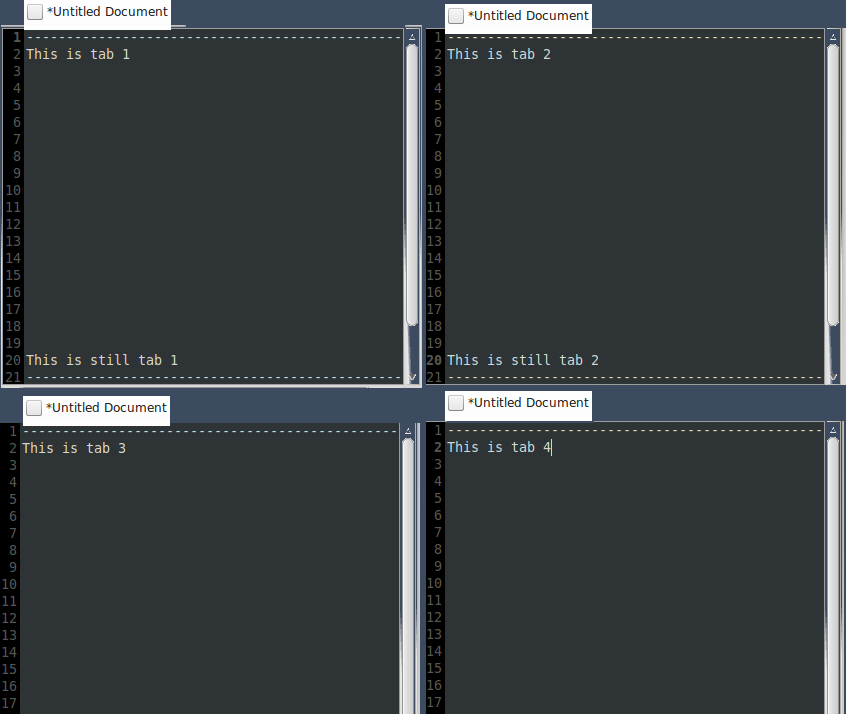
\includegraphics[width=.8\textwidth]{photos/multitasking_tabs.png}
    \caption{Illustration of Multiple Tabs in One Application Window}
    \label{multitasking_tabs}
\end{figure}

The toolbar will also be able to be reorganized according to the user's preference. A locking mechanism will ensure the icons are not accidentally displaced when being used, and the locking mechanism will be toggled by a semi-complex keyboard shortcut, a menu item, or by clicking on the icon of a lock at the edge of the toolbar. The lock icon will be placed to the side, away from the other icons so it is not accidentally toggled. When the lock is clicked, or when the menu item is selected, a pop-up window will ask the user to confirm that the toolbar will become editable. Once in the editable state, the user can click and drag icons or other tools along the toolbars. If no toolbar editing has occured after a set period of time, the toolbar will lock itself unless the user disables this feature in the preferences menu. 

\section{Final Design Layout}
The final design layout will compose of a main document area, similar to that shown in Figure \ref{multitasking_tabs}. Above that area will be a menu toolbar similar to that seen in Figure \ref{Gedit_menu}. The right hand side of each tab will have a scroll bar that appears when the content height becomes larger than the height of the tab, and the left hand side will have numbered lines. The bottom right corner of each tab will have a stretchable icon similar to that of Figure \ref{corner_symbol}. 

\section{Design Analysis}
\subsection{Usability Metrics}
The overall application will measure up against current text editors when considering Nielsen's terminology for the five main ``usability metrics:''  learnability, efficiency, errors, memorability, and satisfaction. 

As the designed interface is a text editor, most users will already have some experience with similar applications and will be able to easily adapt to using the new interface. For the users with text editor experience, the application will be extremely learnable. Their previous experiences will allow them to understand the basics of a text editor so they can immediately begin learning the new features. The new features will be accompanied with tutorials, so that the user can easily step through the features. The tutorial will always be available also, so a user who has not used the application for some time can go back and look through the tutorials to figure out the various features. A user that is inexperienced with text editors will be able to use beginner tutorials that walk them through the purpose and uses of a text editor, the basic tools, and some best practices. When the user feels comfortable with the application, the more advanced tutorials will allow them to learn the more advanced features of the application. The tutorials increase how learnable the application is, and provide the users with a reference on how to use the application.

With multiple forms of input, multiple ways of evoking commands, and customizable user interfaces, the efficiency of the application relates to a user's preferred style of interaction. If they prefer the menus and forms to search for a command, then the user will be less efficient than an individual who chooses to utilize the shortcuts provided by the application. The overall efficiency would remain relatively high, as multiple options are available.

A user's ability to remember how to use the interface would be divided amongst the different features. Features common to text editors are often very basic, and a user would be very likely to remember how to utilize those features. Newer features, like the interface for natural language input, may require a quick glance at a help document or tutorial. This new feature is not typical to other applications, and the user would be less likely to remember the feature's uses after a significant period of time.

Keyboard text input is prone to typing errors, but a natural language input would be able to add content accurately if the user speaks concisely. It is less likely that typing mistakes or misclicks would occur when using natural language styled input, as those devices are not utilized in the process. 

Satisfaction



\subsection{Sytles of Interaction}
This application uses four main styles of interaction: menu, command-line, direct manipulation, and natural language. Menu and command-line interaction styles are common among text editors, whereas direct manipulation and natural language are not as common. The menu aspect is for the toolbars which allow the user to search for commands or tools. They limit the user's need to remember how to use the application, as the tools and commands are laid out for the user to explore easily. The command-line form of interacting is primarily for adding content to a document. The direct manipulation aspect is present in setting the position and size of the application window, the organization of the different tabs, and the organization of the toolbar. 

Direct manipulation gives the user complete control over the elements being moved, improving their satisfaction with the application. If this application were to run on a device with a touch screen, touch inputs would be accepted in the place of mouse clicks, increasing the directness of the user manipulation. The natural language interaction provides the users with an alternative form of adding content to a document. This interaction style will also be used to evoke commands or select tools by utilizing a keyword system. 


%Not sure about the weird spacing of the Xbox citation..
\bibliography{dream_design.bib}{}
\bibliographystyle{plain}

\end{document}



% theories, principles and guidelines
%7 stage sof action, oAI, usability metrics,
%fitt's law, tagazinni's 16, etc
% interaction styles: direct manipulation, menus forms and dialogues, command-line, natural language
% everything together: dream interface, interface that would be as good as possible
% lego exercise: affordance: objects and amterials send you signals, tell you things that help you understand what those things are for
% when it all comes together, the user should get the same picture you had
% 

